\documentclass[11pt,a4paper]{article}
\usepackage{acl2015}
\usepackage{times}
\usepackage[spanish]{babel}
\usepackage[utf8]{inputenc}
\usepackage{url}
\usepackage{latexsym}
\usepackage{graphicx}
\usepackage{floatrow}
\graphicspath{ {images/} }

\DeclareFloatFont{tiny}{\tiny}% "scriptsize" is defined by floatrow, "tiny" not
\floatsetup[table]{font=tiny}

\title{Text Mining II. Diploma de Especialización en Big Data}

\author{Miguel Ángel Sotomayor Fernández \\
  {\tt masfworld@gmail.com} \\}

\date{}

\begin{document}
\maketitle
\begin{abstract}
  El objetivo de este artículo es la generación de un modelo de predicción de la edad y género de las personas en base a unas entradas de texto. Para ello usamos un corpus donde la edad y el género es conocido. La idea principal parte de una bolsa de palabras. Esta BOW se establece analizando todo el corpus. Una vez formada esta BOW, se ordena y se analiza las 1000 primeras con respecto a cada una de las entradas del corpus, calculando su frecuencia de aparición. Partiendo de este trabajo se ha analizado otras posibilidades, en concreto la generación N-gramas en vez de el BOW.
\end{abstract}


\section{Introducción}

El problema de \emph{Author Profiling} se basa en la determinación del género, edad, lenguaje nativo, tipo de personalidad de uno o varios individuos. Este tipo de problema está en auge en muchas areas, tales como las redes sociales y análisis forenses, siendo en este último muy importante para determinan perfiles psicológicos de posibles sospechosos. Otro beneficio podría ser la identificación de los perfiles de los clientes para las empresas.

En este artículo no se pretende introducir una nueva metodología, sino por el contrario, usar diversas técnicas de manera eficiente para la identificación de ciertos parámetros que hagan posible la identificación de un sujeto en base a un texto escrito.



\section{Dataset}

El dataset origen es el conjunto de datos correspondiente al 29 de Abril de 2013 de Pan 13\footnote{http://www.uni-weimar.de/medien/webis/corpora/corpus-pan-labs-09-today/pan-13/pan13-data/pan13-author-profiling-training-corpus-2013-01-09.zip}.

A partir de ests dataset se ha generado una composición de N-gramas de 2 a 5 caracteres. En donde cada uno de esos N-gramas tiene una frecuencia de aparición dentro del corpus original, siendo este nuestro dataset de entrada al algoritmo de predicción. Por tanto, vamos a analizar el dataset correspondiente a los N-gramas y su frecuencia de aparición.

Para el análisis de este dataset se ha usado la herramienta R. El código fuente está dentro de la carpeta R de la solución.

Se va a analizar las medias de la aparición de cada uno de los N-gramas en el corpus. Se van a mostrar los 5 N-gramas más frecuentes:
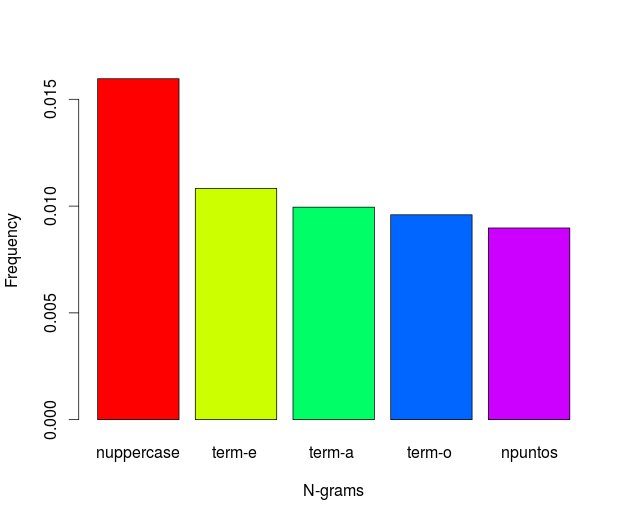
\includegraphics[scale=0.35]{barrasMeans}

Como podemos observar en la gráfica, los N-gramas de vocales comunes en la lengua castellana son muy frecuentes con respecto a otros. "nuppercase",  es una medida adicional a los N-gramas que indica frecuencia de mayúsculas en los textos. "npuntos", es la frecuencia del signo de puntuación "." dentro del texto.


\section{Propuesta del alumno}

Se comenzó analizando la eficiencia de un BOW. Se vio que esta colección de palabras no representaba muy bien ciertos detalles, tales como terminaciones de palabras. 

Por ejemplo, terminaciones como "mente", presente en palabras como ``comunmente, principalmente, seguramente`` pueden ser utilizados por individuos de una determinada franja de edad. Aunque no este el caso, si el estudio se hubiese centrado en el análisis de lugar de procedencia de los individuos, terminaciones como ``ico, ito`` hubieran sido determinantes para establecer el lugar de origen.

Otro aspecto que los N-gramas pueden identificar más claramente que la bolsa de palabras son los géneros, ya que fácilmente identificará frecuencias de aparición en texto de terminaciones como "la, lo".

Hay otras características distintas a los N-gramas que se han tenido en cuentas. En concreto para este trabajo se ha tenido en cuenta las siguientes dimensiones:
\begin{itemize}
\item Frecuencia de comas.
\item Frecuencia de puntos.
\item Frecuencia de dos puntos.
\item Frecuencia de exclamaciones.
\item Frecuencia de interrogaciones.
\item Frecuencia de mayúsculas.
\item Frecuencia de palabras distintas: Para implementar esta característica de manera eficiente, se crea un diccionario donde las claves son todas las palabras de un texto. A continuación se cuenta el número de claves dentro del diccionario.
\item Frecuencia de risas: Se identifica el número de palabras que pueden significar risa, por ejemplo este conjunto \{"jeje", "jaja", "xdd", "hehe", "haha", "jiji", "risa"\}.
\end{itemize}

Para todas estas características se ha calculado su frecuencia con respecto al texto de entrada y se han añadido como dimensión adicional a la frecuencia de N-gramas.

Hay que tener presente los dos tipos de N-gramas. Por un lado tenemos los N-gramas de caracteres y por otro N-gramas de palabras. Por ejemplo, para el caso de las palabras, podemos considerar un trigrama el siguiente texto: "Hola como estas". Para este trabajo hemos considerado que los N-gramas de caracteres podían dar mejores resultados, resultado de unos resultados anteriores a este artículo.

\section{Resultados experimentales}

A continuación se muestra una tabla con los resultados en base a distintas pruebas que se han hecho con diferentes características:

\begin{table}[ht]
\centering
\begin{tabular}{|c|c|c|c|}
\hline
{\bf Técnica} & {\bf Alg. Aprendizaje} & {\bf Age} & {\bf Gender} \\ \hline
N-gramas 3 carac. & Naive Bayes & 53.5172 \% & 49.1054 \% \\ \hline
\begin{tabular}[c]{@{}c@{}}N-gramas 3 carac. + \\ Exclama. e Interrog.\end{tabular} & Naive Bayes & 53.7 \% & 48.8358 \% \\ \hline
\begin{tabular}[c]{@{}c@{}}N-gramas 2-5 carac. + \\ Exclama. e Interrog.\end{tabular} & Naive Bayes & 55.098 \% & 52.6471 \% \\ \hline
\begin{tabular}[c]{@{}c@{}}N-gramas 1-5 carac. +\\ Exclama. e Interrog.\end{tabular} & Naive Bayes & 55.527 \% & 52.5368 \% \\ \hline
\begin{tabular}[c]{@{}c@{}}N-gramas 1-5 carac. \\ +Exclama. e Interrog. +\\ Mayúsculas\end{tabular} & Naive Bayes & 55.6127 \% & 52.5 \% \\ \hline
\begin{tabular}[c]{@{}c@{}}N-gramas 1-5 carac. +\\ Exclama. e Interrog. +\\ Mayúsculas +\\ Distinción Ella-El\end{tabular} & Naive Bayes & 55.6127 \% & 52.5 \% \\ \hline
\begin{tabular}[c]{@{}c@{}}N-gramas 1-5 carac. +\\ Exclama. e Interrog. +\\ Mayúsculas +\\ Distintas palabras\end{tabular} & Naive Bayes & 55.3676 \% & 52.3529 \% \\ \hline
\begin{tabular}[c]{@{}c@{}}N-gramas 1-5 carac. +\\ Exclama. e Interrog. +\\ Mayúsculas +\\ Distintas palabras +\\ Frequencia risas\end{tabular} & Naive Bayes & 56.5441 \% & 52.4142 \% \\ \hline
\begin{tabular}[c]{@{}c@{}}N-gramas 1-5 carac. +\\ Exclama. e Interrog. +\\ Mayúsculas +\\ Distintas palabras\end{tabular} & Super Vector Machine & 63.025 \% & 59.4363 \% \\ \hline
\begin{tabular}[c]{@{}c@{}}N-gramas 2-5 carac. +\\ Exclama. e Interrog. +\\ Mayúsculas +\\ Frequencia risas\end{tabular} & Super Vector Machine & 63.076 \%  &  \\ \hline
\end{tabular}
\caption{Resultados (\emph{Accuracy})}
\label{my-label}
\end{table}

Todas las pruebas llevan implícitas las siguientes características:
\begin{itemize}
\item Frecuencia de comas
\item Frecuencia de puntos
\item Frecuencia de dos puntos
\end{itemize}

Se puede observar que la inclusión de los N-gramas supone un aumento ``considerable" del \emph{accuracy}. Las demás características no aportan mucho, algunas mejoran un poco, pero no es considerable el aumento, salvo la frecuencia de risas.

Como era de esperar si cambiamos un algoritmo probabilístico, como es el "Naive Bayes", por un Super Vector Machine mejoramos notablemente.

La última prueba, la cual se considera más satisfactoria , contiene las siguientes características:
\begin{itemize}
\item N-gramas entre 2 y 5 caracteres
\item Frecuencia de comas
\item Frecuencia de puntos
\item Frecuencia de dos puntos
\item Frecuencia de exclamaciones e interrogaciones
\item Frecuencia de mayúsculas
\item Frecuencia de risas
\end{itemize}

\section{Conclusiones y trabajo futuro}

Se ha podido observar que los N-gramas son un buen punto de partida a la hora de realizar ``Author profiling". Sin embargo todavían quedan múltiples características a explorar y modelos que generar.

En el futuro sería recomendable probar a mezclar en un mismo dataset N-gramas de caracteres y de palabras, para más tarde aplicar un algoritmo PCA de reducción de dimensiones.


\begin{thebibliography}{}

\bibitem[\protect\citename{Rangel and Rosso}2014]{Aho:2014}
F. Rangel, P. Rosso, I. Chugur, M. Potthast, M. Trenkmann, B. Stein, B. Verhoeven, W, Daelemans.
\newblock 2014.
\newblock {\em Overview of the 2nd Author Profiling Task at PAN 2014}

\bibitem[\protect\citename{Soler}2013]{Aho:2013}
Juan Soler Company
\newblock 2013.
\newblock {\em Author Profiling:Gender Identification}

\end{thebibliography}

\end{document}
